%!TEX program = xelatex



\documentclass[cn,black,10pt,normal]{elegantnote}
\usepackage{float}
\usepackage{hyperref}


%\newcommand{\upcite}[1]{\textsuperscript{\textsuperscript{\cite{#1}}}}

\title{数码摄影作业(11)后期镜头矫正}
\author{姓名:姜文渊\\学号:1951510}
%\institute{School of Life Science, Tongji University}
%\version{1.00}
\date{2021年5月23日}

\begin{document}

\maketitle

\section{调整前的图片}

\begin{figure}[H]
    \centering
    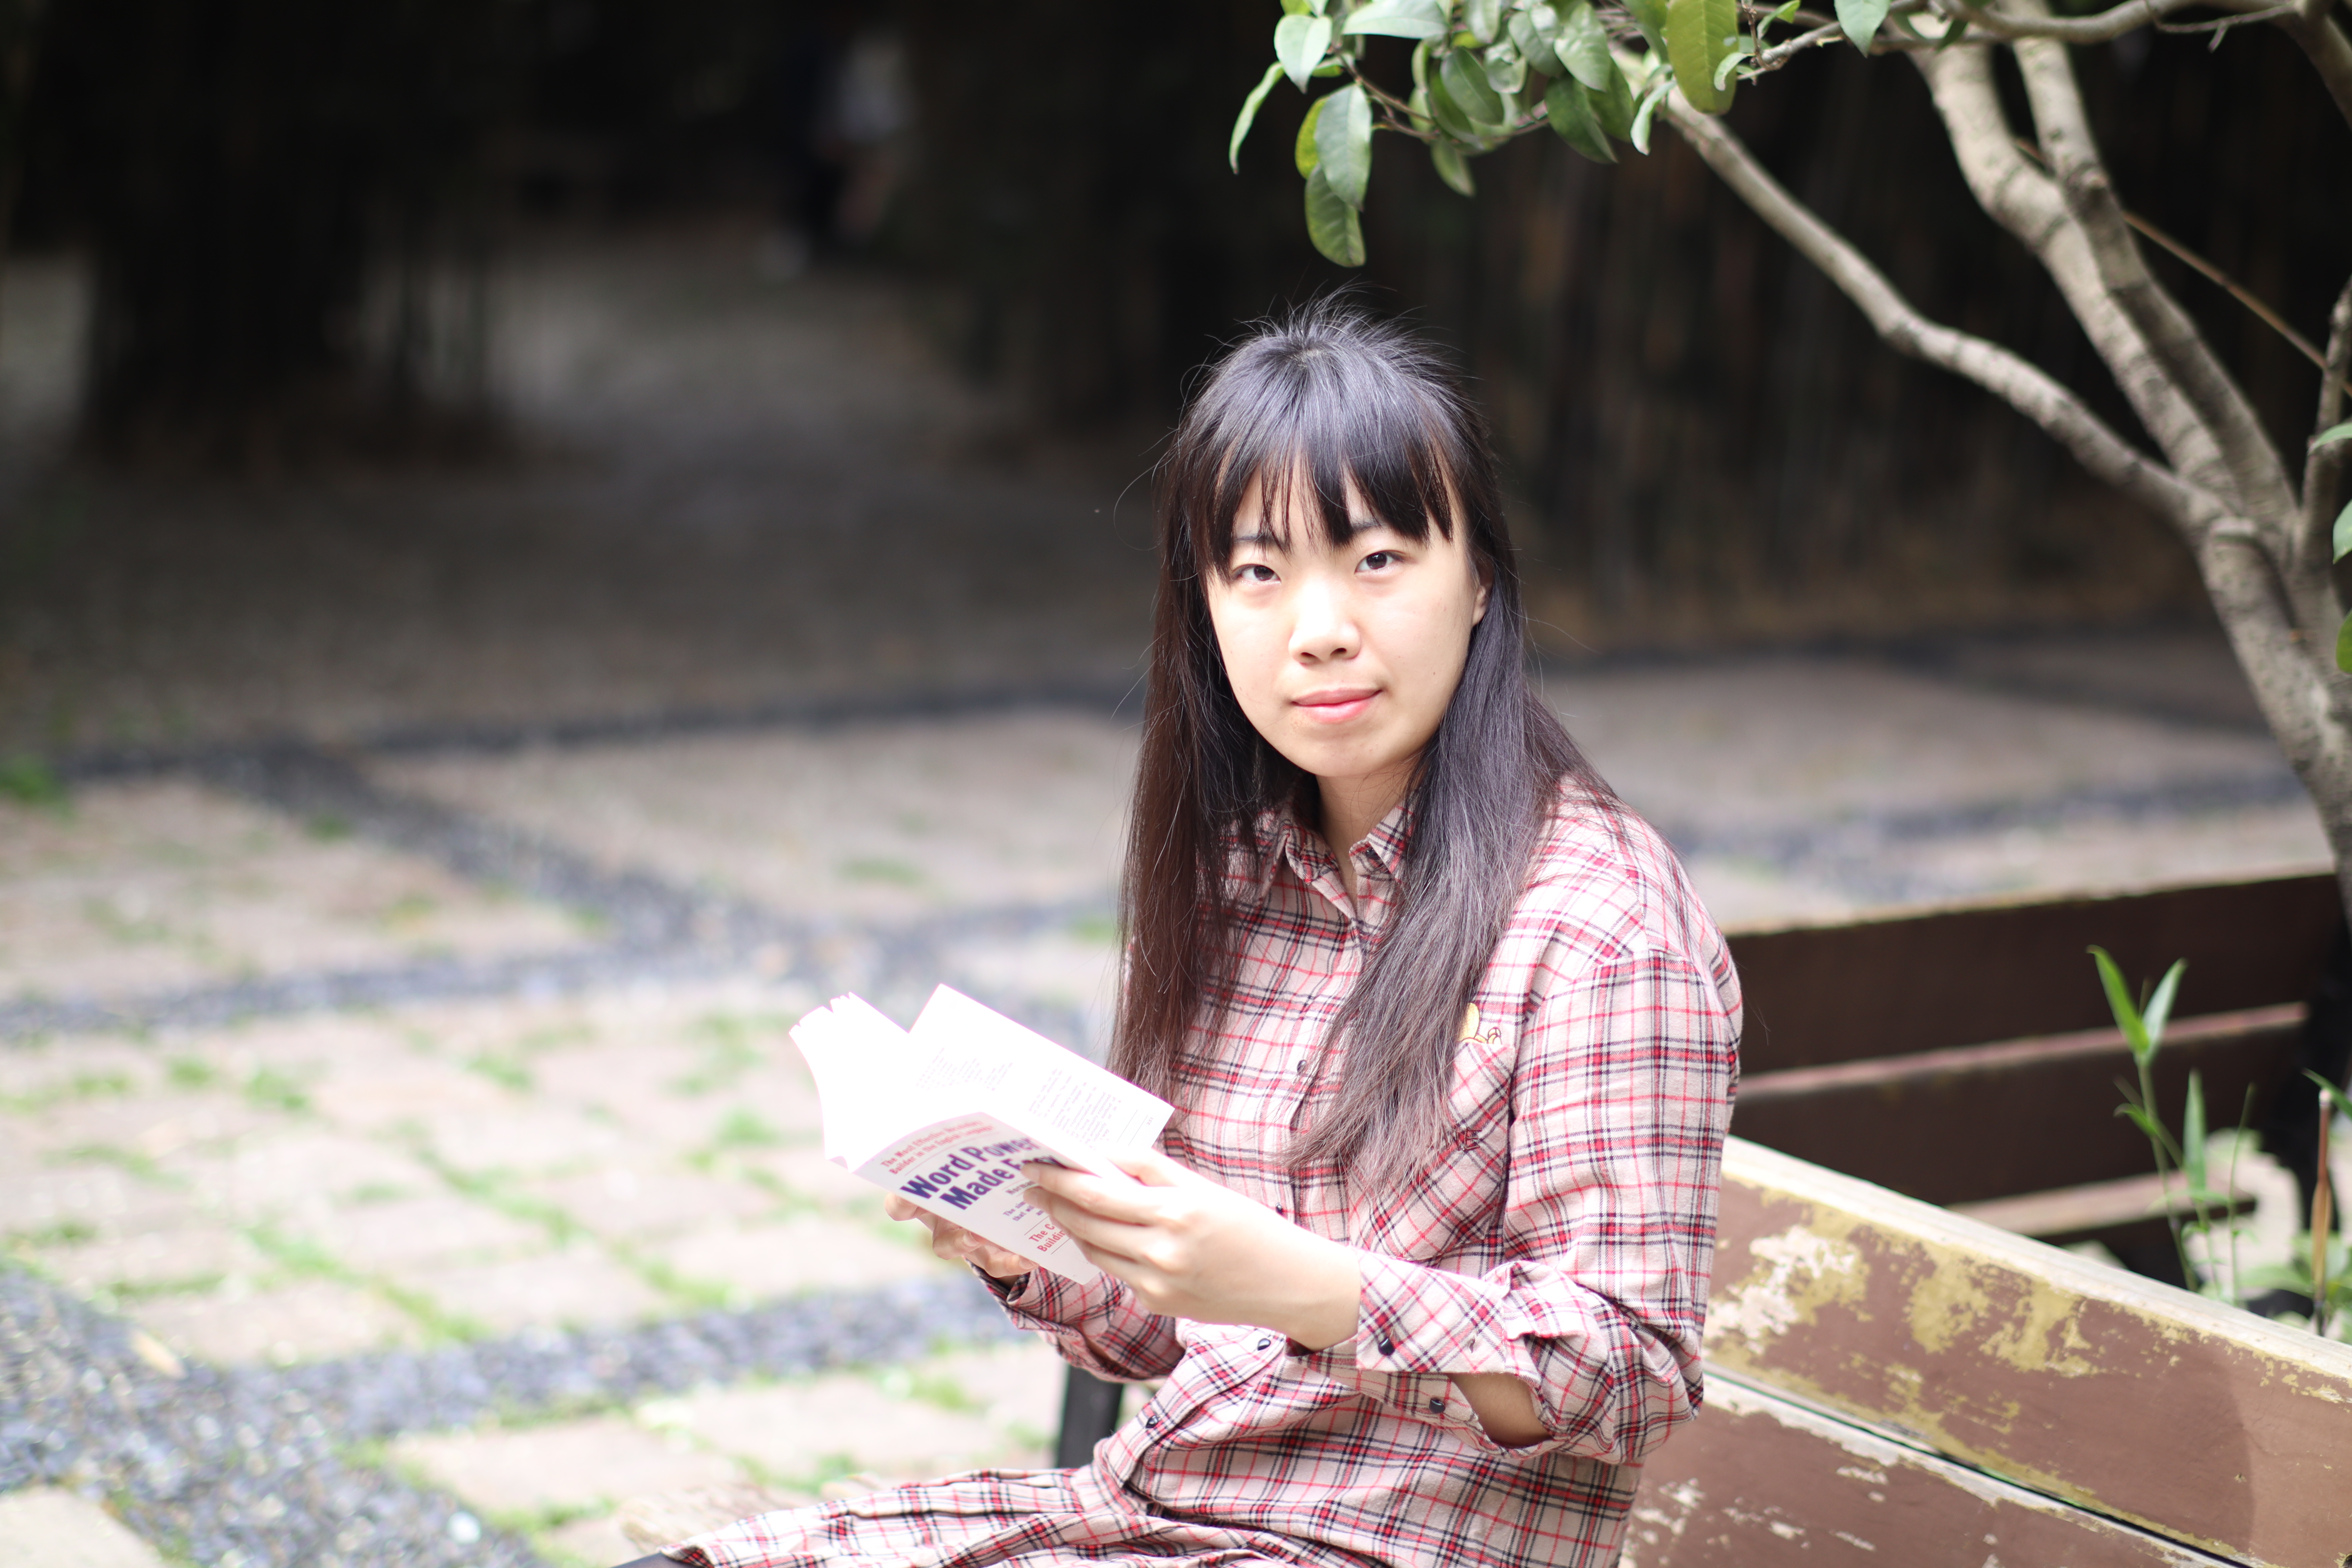
\includegraphics[width=0.5\textwidth]{F1}
    %\caption{From “Pacific Theater,” WWII, 1942-45 \\ 路易斯·蒙巴顿勋爵上将在萨拉托加号上向人员致辞}
    \label{F-02}
\end{figure}

该图片拍摄于圣母百花大教堂,由彩色玻璃窗构成,由于拍摄时的设备(佳能卡片机)和位置所限,故无法拍出正面的玻璃窗上的图案。

\section{调整后的图片}

\begin{figure}[H]
    \centering
    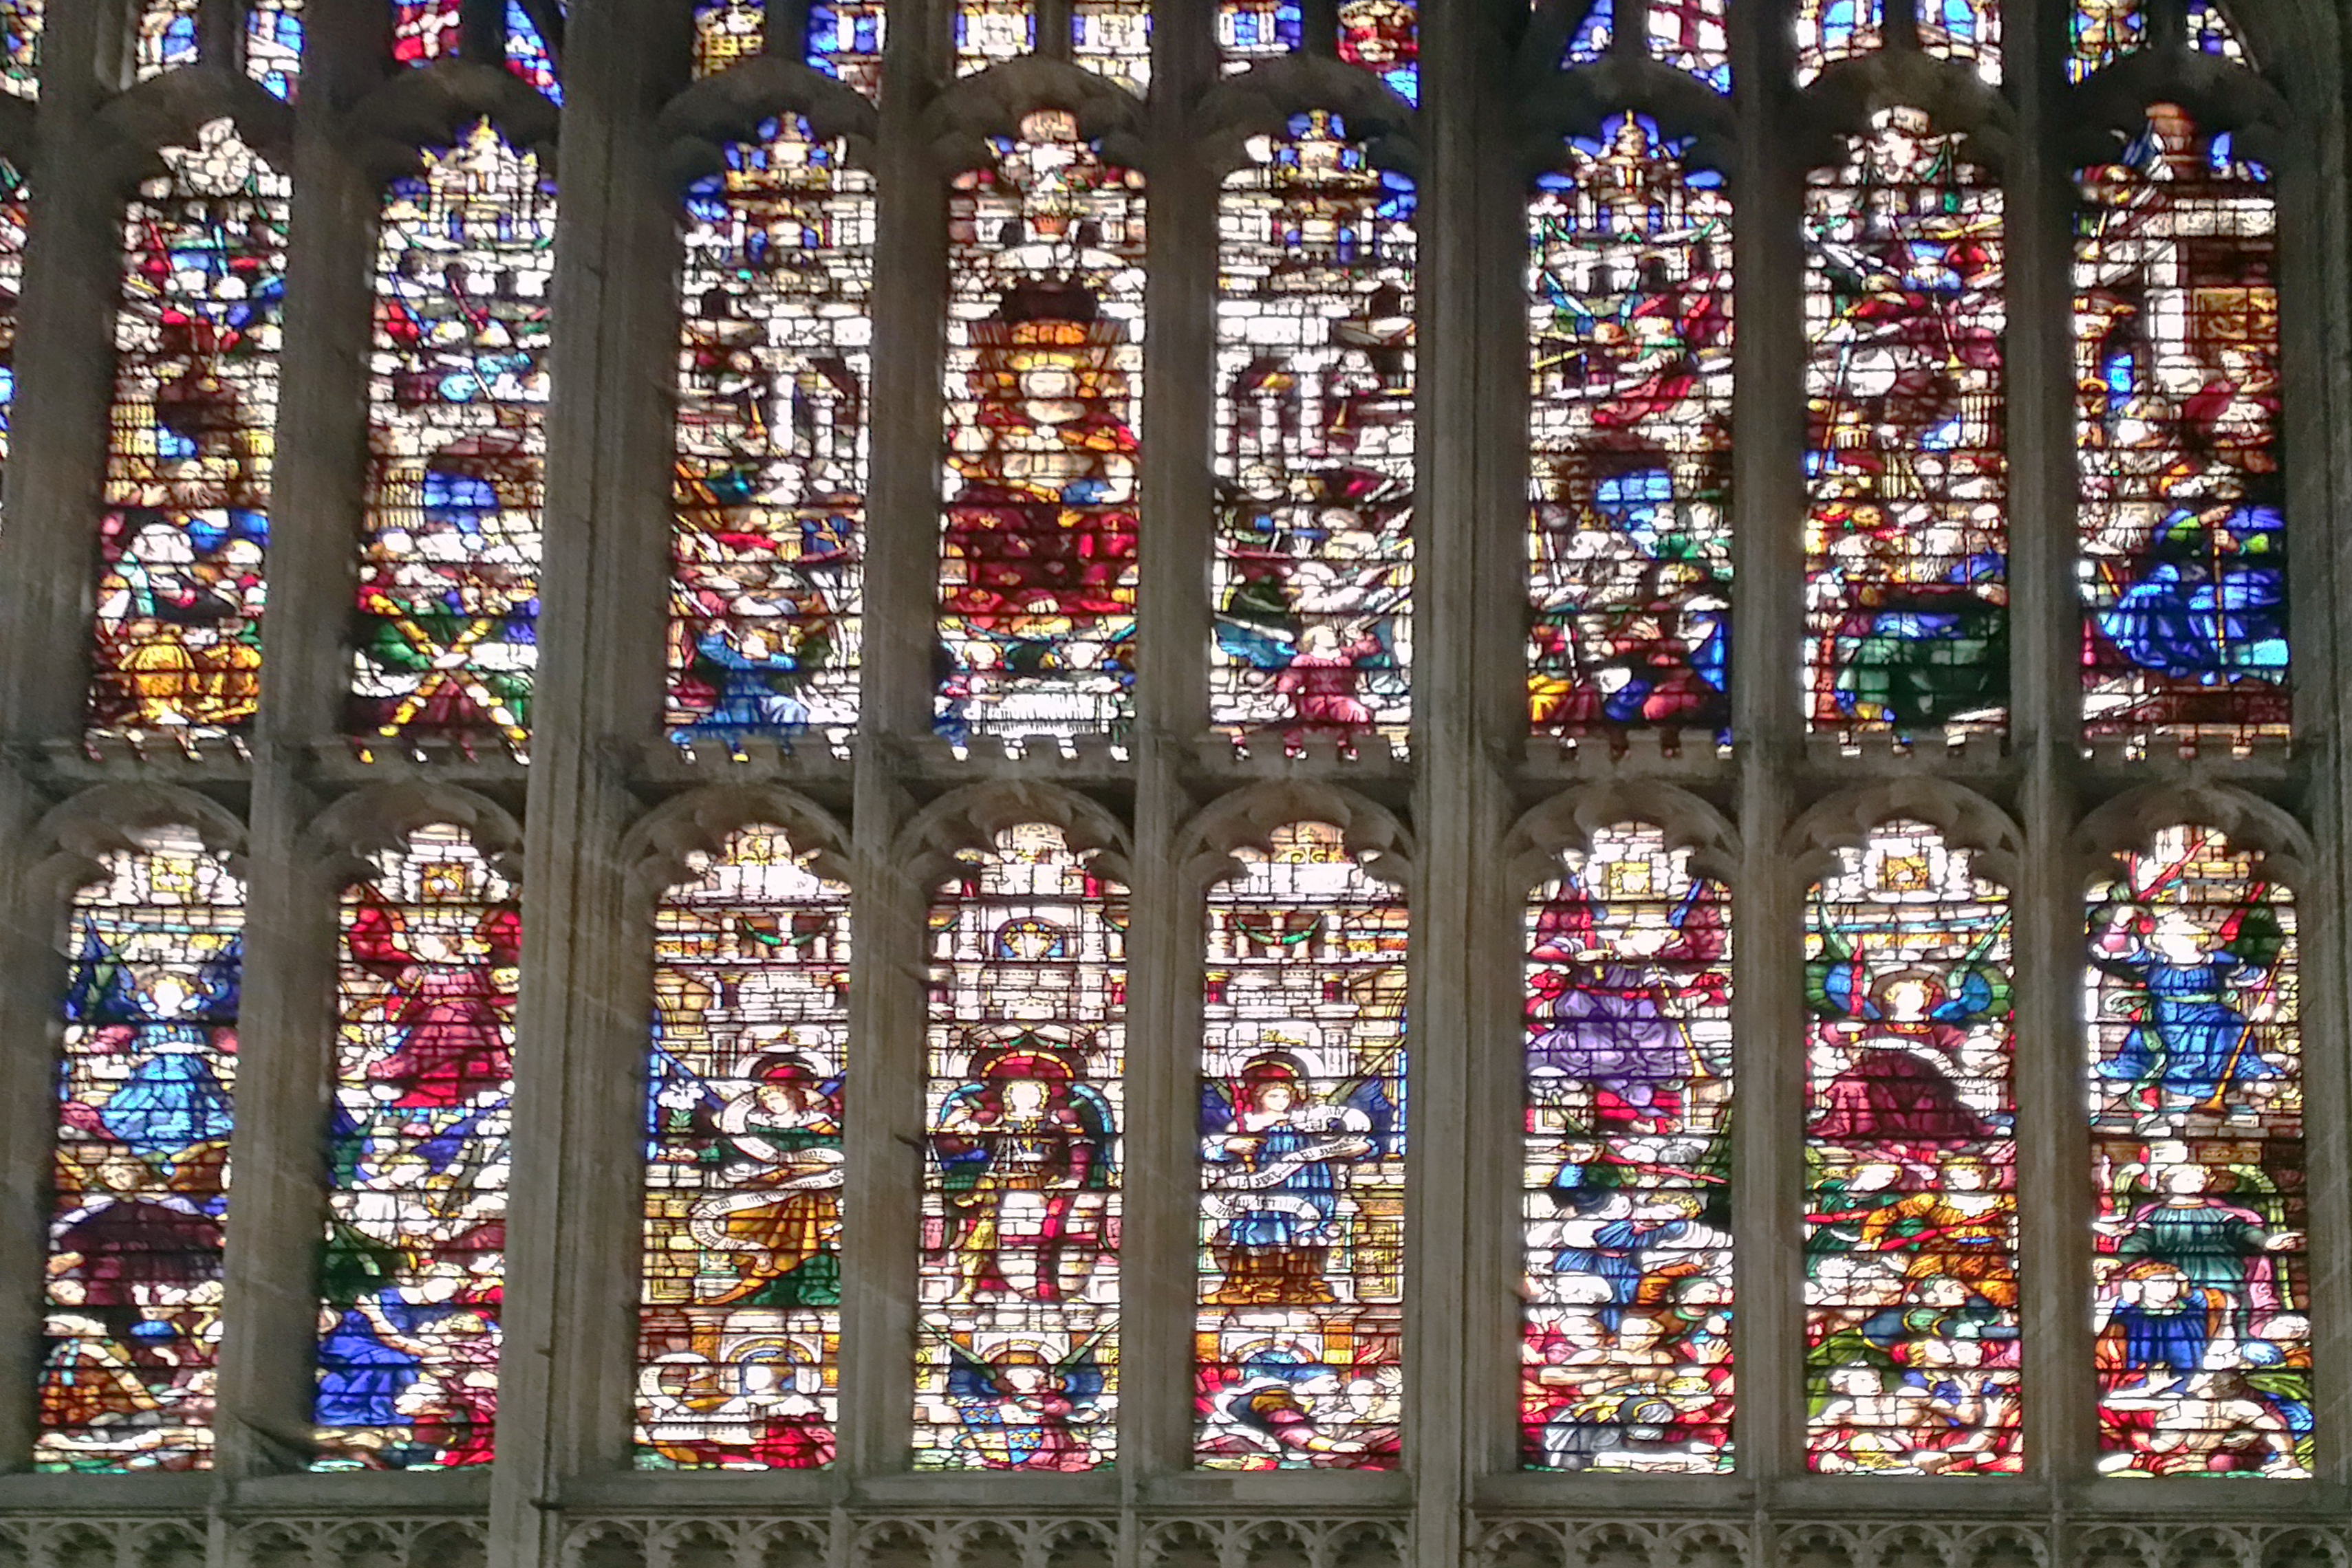
\includegraphics[width=0.5\textwidth,angle=0]{F2}
    %\caption{From “Pacific Theater,” WWII, 1942-45 \\ 士兵受伤流血的手}
    \label{F-01}
\end{figure}

经过镜头矫正,裁剪,调整色彩曲线后,图像视野大幅度减少,但是可以看见规整的彩色玻璃窗上几乎未变形的图案。


%\bibstyle{unsrt}
%\bibliography{references}{}
\end{document}
